\documentclass[12pt]{article}
\usepackage[spanish]{babel}
\usepackage[utf8]{inputenc}
\usepackage[T1]{fontenc}
\usepackage{geometry}
\usepackage{listings}
\usepackage{mdframed}
\usepackage{amsmath, amssymb, amsfonts, amsthm}
\usepackage{graphicx}
\usepackage{fancyhdr, colortbl}
% paquete para includegraphics
\usepackage{graphicx}
\usepackage{tcolorbox}
\usepackage{tabularx}
\usepackage{array}
\usepackage{colortbl}
\tcbuselibrary{skins}
\usepackage{xcolor}

\pagestyle{fancy}
\fancyhf{} % Limpia los encabezados y pies de página
\fancyhead[L]{Pedro Villar} % Encabezado en la parte izquierda

\definecolor{darkcyan}{HTML}{0091A4}
\definecolor{brightcyan}{HTML}{dcf0f2}  

\newmdenv[
topline=false,
rightline=false,
bottomline=false,
leftline=true,
linecolor=darkcyan,
linewidth=3pt,
backgroundcolor=brightcyan,
frametitle=Respuesta
]{rta}

\newcolumntype{Y}{>{\centering\arraybackslash}X}
  \tcbset{tab2/.style={enhanced,fonttitle=\bfseries,fontupper=\normalsize\sffamily,
  colback=white!10!white,colframe=blue!50!black,colbacktitle=blue!40!white,
  coltitle=black,center title}}

\geometry{margin=1.9cm}

\lstdefinestyle{CStyle}{
    language=C,                      % El lenguaje a usar
    basicstyle=\ttfamily\small,      % Tipo de fuente
    keywordstyle=\color{blue},       % Color de palabras clave
    commentstyle=\color{green},      % Color de comentarios
    stringstyle=\color{red},         % Color de strings
    numberstyle=\tiny\color{gray},   % Estilo de los números de línea
    numbers=left,                    % Colocar los números de línea a la izquierda
    stepnumber=1,                    % Numerar todas las líneas
    numbersep=10pt,                  % Separación entre los números de línea y el código
    tabsize=4,                       % Tamaño de las tabulaciones
    showspaces=false,                % No mostrar los espacios como caracteres especiales
    showstringspaces=false,          % No mostrar los espacios en las cadenas de texto
    breaklines=true,                 % Hacer saltos de línea automáticos
    frame=single,                    % Cuadro alrededor del código
}

\lstdefinestyle{BashStyle}{
    language=bash,                    % El lenguaje a usar
    basicstyle=\ttfamily\small,       % Tipo de fuente
    keywordstyle=\color{blue},        % Color de palabras clave (comandos de bash)
    commentstyle=\color{green},       % Color de comentarios
    stringstyle=\color{red},          % Color de cadenas (strings)
    numberstyle=\tiny\color{gray},    % Estilo de los números de línea
    numbers=left,                     % Colocar los números de línea a la izquierda
    stepnumber=1,                     % Numerar todas las líneas
    numbersep=10pt,                   % Separación entre los números de línea y el código
    tabsize=4,                        % Tamaño de las tabulaciones
    showspaces=false,                 % No mostrar espacios especiales
    showstringspaces=false,           % No mostrar espacios en las cadenas de texto
    breaklines=true,                  % Hacer saltos de línea automáticos
    frame=single,                     % Colocar un cuadro alrededor del código
    morekeywords={echo, cd, ls, rm, mkdir}, % Añadir palabras clave de bash
}

\begin{document}

\section*{Práctico 4 - Persistencia}

\noindent \textit{Ejercicio 1.} Ejercicio 1. El disco Seagate Exos 7E8 de 8 TiB e intefaz SAS tiene una velocidad de rotación de $7200 \mathrm{RPM}, 4.16 \mathrm{~ms}$ de latencia de búsqueda y $215 \mathrm{MiB} / \mathrm{s}$ de tasa de transferencia.

\begin{itemize}
    \item[(a)] Indicar cuantos $m s$ tarda en dar una vuelta completa.
    \item[(b)] Indicar la tasa de transferencia de lectura al azar de bloques de 4096 bytes.
\end{itemize}

\begin{rta}
    \begin{itemize}
        \item[(a)] Cálculo de tiempo rotacional:
        \begin{equation*}
            T_{rotacional} = \frac{60}{7200} \cdot 1000 = 8.33 \mathrm{ms}
        \end{equation*}
        \item[(b)] Para la tasa de transferencia de E/S al azar de un bloque de 4096 bytes, se debe calcular lo siguiente:
        \begin{equation*}
            R_{I/O} = \frac{SIZE_{Transfer}}{T_{I/O}} = \frac{4096}{....}
        \end{equation*}
        Debo calcular el tiempo de transferencia:
        \begin{align*}
            T_{I/O} &= T_{seek} + T_{rotacional} + T_{transfer} \\
            T_{I/O} &= 4.16 + 4.16 + \frac{4096}{215 \cdot 2^{20}} \cdot 1000 \\
            &= 4.16 + 4.16 + 0.01817 = 8.3382 \mathrm{ms}
        \end{align*}
        Por lo tanto, la tasa de transferencia de lectura al azar de bloques de 4096 bytes es de:
        \begin{equation*}
            R_{I/O} = \frac{4096}{8.3382} = 491.2331 \mathrm{KiB/ms}
        \end{equation*}
    \end{itemize}
\end{rta}

\noindent \textit{Ejercicio 2.} Compute el tamaño de la FAT para:

\begin{itemize}
    \item[(a)] Un diskette de doble cara doble densidad 360 KiB ( 1982): FAT12, cluster ${ }^{\text {P }}$ de 512 bytes.
    \item[(b)] Un disco duro de 4 GiB ( 1998): FAT16, cluster de 4096 bytes.
    \item[(c)] Un pendrive 32 GiB ( 2014): FAT32, cluster de 16384 bytes.
\end{itemize}

\begin{rta}
    \begin{itemize}
        \item[(a)] El tamaño de la FAT para un diskette de doble cara doble densidad de 360 KiB es:
        \begin{equation*}
            \text{FATSize} = \underbrace{\frac{360 \cdot 1024}{512}}_{\text{cant de clusters}} \cdot \underbrace{12 \text{bits/cluster}}_{FAT entry} = 720 \cdot 1.5 = 8640 \text{ bits} = 1080 \text{ bytes}
        \end{equation*}
        \item[(b)] El tamaño de la FAT para un disco duro de 4 GiB es:
        \begin{equation*}
            \text{FATSize} = \underbrace{\frac{4 \cdot 1024^3}{4096}}_{\text{cant de clusters}} \cdot \underbrace{16 \text{bits/cluster}}_{FAT entry} = \frac{2^2 \cdot 2^{30}}{2^2 \cdot 2^{10}} \cdot 2^1 = 2^21 = 2 \text{ MiB} 
        \end{equation*}
        \item[(c)] El tamaño de la FAT para un pendrive de 32 GiB es:
        \begin{equation*}
            \text{FATSize} = \underbrace{\frac{32 \cdot 1024^3}{16384}}_{\text{cant de clusters}} \cdot \underbrace{32 \text{bits/cluster}}_{FAT entry} = \frac{2^5 \cdot 2^{30}}{2^4 \cdot 2^{10}} \cdot 2^2 = 2^23 = 8 \text{ MiB}
        \end{equation*} 
    \end{itemize}
\end{rta}

\noindent \textit{Ejercicio 3.} El sistema de archivos de xv6 es una estructura la Fast-Filesystem for UNIX (UFS), con parámetros: bloque de 512 bytes, 12 bloques directos, 1 bloque indirecto, índices de bloque de 32 bits.

\begin{itemize}
    \item[(a)] Calcule el tamaño máximo de un archivo.
    \item[(b)] Calcule el tamaño de la sobrecarga para un archivo de tamaño máximo.
    \item[(c)] ¿Se podrían codificar los números de bloque con menos bits? ¿Qué otros efectos produciría utilizar la mínima cantidad de bits?
\end{itemize}

\begin{rta}
    \begin{itemize}
        \item[(a)] \textbf{Tamaño máximo:} el que usa todos los bloques directos y el indirecto.
        \begin{equation*}
            \text{MaxFileSize} = \underbrace{512 \cdot 12}_{\text{b. directos}} + \underbrace{512\cdot \frac{512}{4}}_{\text{b. indirectos}} = 512 \cdot \left(12 + \frac{512}{4}\right) = 512 \cdot (12 + 128) =70KiB
        \end{equation*}
        
        \item[(b)] Como hay un único bloque indirecto y el tamaño de bloque es de 512 bytes, la sobrecarga es simplemente 512 bytes.
        
        \item[(c)] Si usas la mínima cantidad de bits, hay menos bloques redireccionables, data bitmap mas chico, tamaño máximo de archivo más grande. 
        
        \item[(E)] Modificar los parámetros de forma que pueda duplicar el tamaño máximo de un archivo: 
        \begin{itemize}
            \item Duplicar el tamaño de bloque, el tamaño máximo de archivo va a ser:
            \begin{equation*}
                \text{MaxFileSize} = 1024 \cdot \left(12 + \frac{1026}{4}\right) = 1024 \cdot (12 + 512)
            \end{equation*}
            \textit{El archivo va a ser mucho mas que el doble, no es una solución directa.}
            \item Dividir en 2 el tamaño del índice de bloques, el tamaño máximo de archivo va a ser:
            \begin{equation*}
                \text{MaxFileSize} = 512 \cdot \left(12 + \frac{512}{2}\right) = 512 \cdot (12 + 256)
            \end{equation*}
            \textit{El archivo es menos del doble de tamaño.}
            \item Duplicar la cantidad de bloques directos e indirectos.
        \end{itemize}
        \item[(E2)] ¿El tamaño máximo de archivo, es equivalente a la cantidad máxima de todos los archivos que puedo almacenar en ese file system? Como con un archivo no podemos llenar todo el disco duro por lo pronto sabemos que el tamaño máximo de todos los archivos que puedo almacenar es mayor.
        \begin{equation*}
            \text{dataRegion} = 512 \cdot 2 ^{32} = 2^9 \cdot 2^{32} = 2^{41} = 2 TiB
        \end{equation*}
        
    \end{itemize}
\end{rta}

\noindent \textit{Ejercicio 4.} Para un sistema de archivos xv6: bloque de 512 bytes, 12 bloques directos, 1 bloque indirecto, índices de bloque de 32 bits.

\begin{itemize}
    \item[(a)] Indique que número de bloque hay que leer para acceder al byte 451, al byte 6200 y al byte 71000 .
    \item[(b)] Dar la expresión matemática que indica a partir del byte que número de bloque hay que acceder. Se puede usar división por casos, ejemplo positivo $(x)=\mathbf{1}$ si $0<x, \mathbf{0}$ si $x \leq 0$.
\end{itemize}

\begin{rta}
    \textbf{Punto a:} Para acceder al byte 451, se necesita el \textbf{índice directo 0}, luego para acceder al byte 6200 y 7200 debería hallar las ubicaciones:
    \begin{itemize}
        \item En total son 12 bloques directos, es decir cubro primero 6144B, pero esto no me alcanza, por lo que debería acceder al bloque contiguo al último bloque directo, es decir a lo que apunta el bloque indirecto (\textbf{*índice indirecto 0}).
        \item Luego si quiero acceder al byte 71000, deberia hallar el puntero del bloque indirecto que apunte al bloque físico que contiene el byte 71000, para ello hago la siguiente cuenta: primero le saco los bloques indirectos $71000-12\cdot 512 = 64856$, y ahora busco que puntero indirecto es el que necesito $\frac{64856}{512}=126$ por lo que necesito el \textbf{*índice indirecto 126}. 
    \end{itemize}
    \textbf{Punto b:} La expresión matemática que indica a partir del byte que número de bloque hay que acceder es:
    \begin{equation*}
        \text{indexOfBlock}(x) =
        \begin{cases}
            \frac{x}{512} & \text{si } x \leq 12 \cdot 512 \\
            \frac{x - 12 \cdot 512}{512} & \text{en caso contrario }
        \end{cases}
    \end{equation*}
\end{rta}

\noindent \textit{Ejercicio 5.} Considere un disco de 16 TiB ( $2^{44}$ bytes) con bloques de 4 KiB ( $2^{12}$ bytes) e índices de bloque de 32 bits. Suponga que el sistema de archivos esta organizado con i-nodos de hasta 3 niveles de indirección y hay 8 punteros a bloques directos. ¿Cuál es el máximo tamaño de archivo soportado por este sistema de archivos? Justifique su respuesta.

\begin{figure}[h]
    \centering
    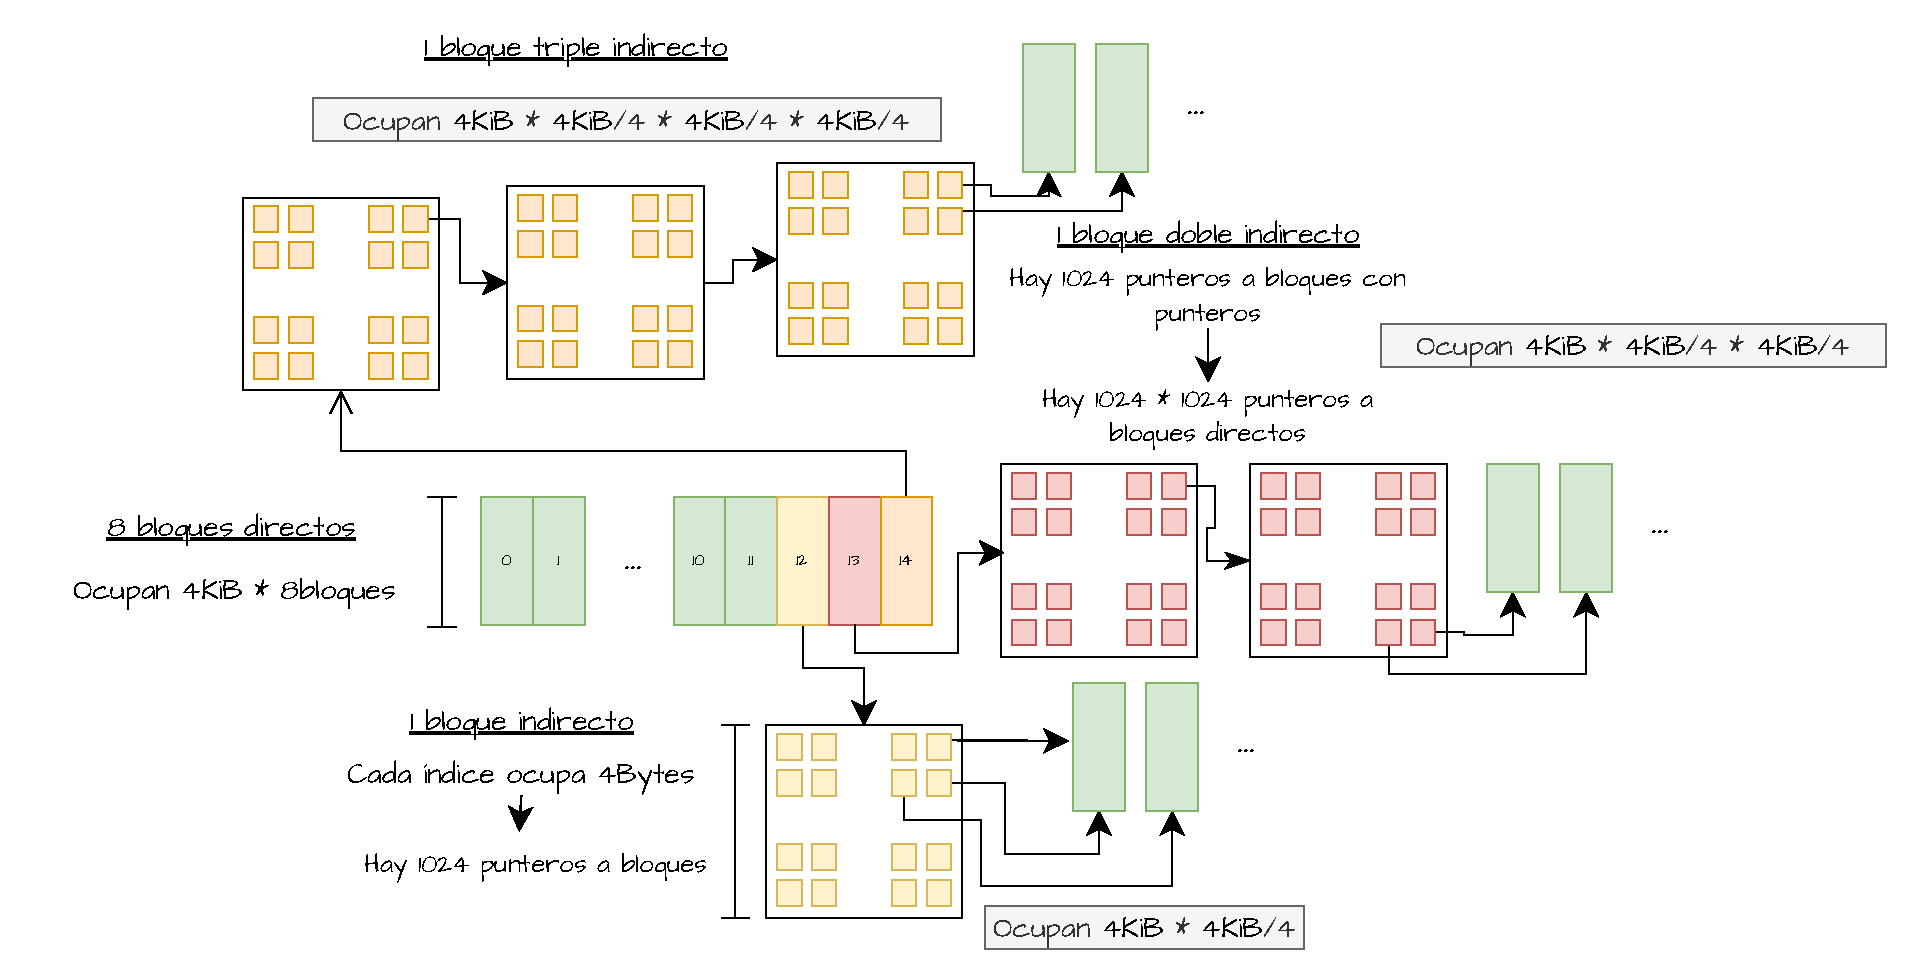
\includegraphics[width=1\textwidth]{ej5.pdf}
\end{figure}

\newpage
\begin{rta}
    \textbf{Tamaño máximo:} el que usa todos los bloques:
    \begin{equation*}
        \text{MaxFileSize} = \underbrace{4096 \cdot 8}_{\text{b. directos}} + \underbrace{4096 \cdot \frac{4096}{4}}_{\text{b. indirecto}} + \underbrace{4096 \cdot \left(\frac{4096}{4}\right)^2}_{\text{b. doble indirecto}} + \underbrace{4096 \cdot \left(\frac{4096}{4}\right)^3}_{\text{b. triple indirecto}} = 4TiB
    \end{equation*}
\end{rta}

\noindent \textit{Ejercicio 6.} Considere el sistema de archivos de xv6. \newline Indique que bloques directos o indirectos hay que crear. Suponga que el i-nodo ya está creado en disco. Puede usar esquemas.

\begin{itemize}
    \item[(a)] Se crea un archivo nuevo y se agregan 6000 bytes.
    \item[(b)] Se agregan al final 1000 bytes más.
\end{itemize}


\begin{rta}
    Para este ejercicio, el file system de xv6 tiene \textbf{12 bloques directos} y \textbf{1 indirecto}. Al agregarle 6000 bytes se van a necesitar $\frac{6000}{512} = 12$ bloques, por lo que suponiendo que tenemos el i-nodo creado, se van a necesitar los 12 bloques directos. Luego, al agregar 1000 bytes más, se necesitará un bloque más, por lo que se va a necesitar el bloque indirecto para acceder a dos bloques más.
\end{rta}

\noindent \textit{Ejercicio 7.} Supongamos que se borró todo el mapa de bits con los bloques en uso de un filesystem tipo UNIX. Explique el procedimiento para recuperarlo.


\begin{rta}
    El proceso sería el siguiente:
    \begin{itemize}
        \item Recorrer todos los i-nodos y marcar los bloques que están en uso.
    \end{itemize}
\end{rta}

\noindent \textit{Ejercicio 8.} Un programa que revisa la estructura del filesystem (fsck) con el método del ejercicio anterior construyó la siguiente tabla de bloques que aparecen en uso vs. bloques que se indican como libres en el bitmap del disco.  

\begin{figure}[h]
    \centering
    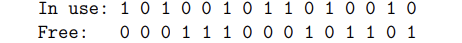
\includegraphics[width=0.5\textwidth]{d1.png}
\end{figure}

¿Hay errores? De ser así ¿resultan importantes?\\
Ayuda: analice los 4 casos posibles y discuta cada uno.


\begin{rta}
    Hay errores ya que algunos lugares están marcados como ocupados cuando estan libres o están ocupados y no están marcados de tal manera. Las posibilidades son las siguientes:
    \begin{itemize}
        \item \textbf{00}: Este caso representa que no está en uso pero no está libre, eso indica que hay no hay inodo que ocupe ese bloque entonces lo marcamos en el d-bmap como 1, diciendo que está libre.
        \item \textbf{01}: Este caso está bien, ya que no está en uso y está libre.	
        \item \textbf{11}: Este caso representa que está en uso y está libre, lo cual es un error ya que no puede estar en uso y libre al mismo tiempo. Entonces, se debe marcar como ocupado en el bitmap.
        \item \textbf{10}: Este caso está bien, está en uso y no está libre.
    \end{itemize}
\end{rta}

\noindent \textit{Ejercicio 9.} Suponiendo a) no hay nada en la caché de bloques de disco, b) cada consulta a un i-nodo genera exactamente una lectura de bloque, c) cada directorio entra en un bloque, d) cada archivo también entra en un bloque. Describa la secuencia de lecturas de bloque para acceder a los archivos:

\begin{itemize}
    \item[(a)] /initrd.img
    \item[(b)] /usr/games/moon-buggy
\end{itemize}

\begin{rta}
    \begin{itemize}
        \item[(a)] Lectura de bloques para acceder a /initrd.img \textbf{4 lecturas de bloque}:
        \begin{enumerate}
            \item \textbf{Read} el inodo de la carpeta raíz \texttt{/}. Para buscar dentro de sus datos, el puntero al inode de initrd.img.
            \item \textbf{Read} los datos de la carpeta raízz buscando efectivamente al archivo.-
            \item \textbf{Read} el inodo del archivo \texttt{initrd.img}.   
            \item \textbf{Read} los datos del archivo.
        \end{enumerate} 
        \item[(b)] Lectura de bloques para acceder a /usr/games/moon-buggy \textbf{8 lecturas de bloque}:
        \begin{enumerate}
            \item \textbf{Read} el inodo de la carpeta raíz \texttt{/}. Para buscar dentro de sus datos, el puntero al inode de usr.
            \item \textbf{Read} los datos de la carpeta raíz buscando efectivamente al archivo de tipo directorio usr.
            \item \textbf{Read} el inodo de la carpeta \texttt{usr}. Para buscar dentro de sus datos, el puntero al inode de games.
            \item \textbf{Read} los datos de la carpeta usr buscando efectivamente al archivo de tipo directorio games.
            \item \textbf{Read} el inodo de la carpeta \texttt{games}. Para buscar dentro de sus datos, el puntero al inode de moon-buggy.
            \item \textbf{Read} los datos de la carpeta games buscando efectivamente al archivo de tipo archivo moon-buggy.
            \item \textbf{Read} el inodo del archivo \texttt{moon-buggy} para obtener los metadatos de los permisos, y poder acceder a sus datos.
            \item \textbf{Read} los datos del archivo moon-buggy.
        \end{enumerate}
    \end{itemize}
\end{rta}

\noindent \textit{Ejercicio 10.} Un novato en diseño e implementación de sistemas de archivos sugiere que la primera parte del contenido de cada archivo UNIX se almacene en el i-nodo mismo. ¿Es una buena idea? Explique.

\begin{rta}
    En general, \textbf{no es una buena idea} ya que los i-nodos están diseñados principalmente para almacenar \textbf{metadatos} y manejar eficientemente archivos de cualquier tamaño. Sin embargo, en sistemas donde predominan los archivos pequeños y el acceso rápido es crítico, esta técnica podría tener ciertas ventajas.
    \newline \texttt{Ventajas:}
    \begin{itemize}
        \item Acceso mas rápido en archivos muy chicos. Reduciría la latencia en operaciones con archivos muy chicos.
        \item Devuelta si los archivos son muy chicos,  se evitaría la asignación de bloques en el disco para almacenar datos mínimos. Esto podría ahorrar espacio y simplificar la administración de bloques.
    \end{itemize}
    \texttt{Desventajas}
    \begin{itemize}
        \item Los i-nodos tienen un tamaño fijo y limitado. Si parte de este espacio se dedica a almacenar contenido, se reduciría la cantidad de metadatos que puede almacenar, como punteros a bloques, atributos extendidos, o tiempo de acceso/modificación.
        \item Aumento de complejidad en algoritmos. Los algoritmos para manejar esta dualidad (contenido directo en el i-nodo versus en bloques de disco) serían más complicados, ya que habría que decidir si un archivo debe usar solo el i-nodo o también bloques externos.
    \end{itemize}
\end{rta}

\newpage
\noindent \textit{Ejercicio 11.} El campo link count dentro de un i-nodo resulta redundante. Todo lo que dice es cuantas entradas de directorios apuntan a ese i-nodo, y esto es algo que se puede calcular recorriendo el grafo de directorios. ¿Por qué se usa este campo?

\begin{rta}
    Al hacer \texttt{unlink}, si no tuviesemos ese campo, se debería recorrer todo el sistema de archivos por cada llamada, y sería muy poco eficiente. Por lo que este campo nos ahorra recursos en el manejo de los links.
\end{rta}

\noindent \textit{Ejercicio 12.} Ya vimos que las estructuras de datos en disco de los FS mantienen información redundante que debería ser consistente. Piense en más pruebas de consistencia de debería realizar un filesystem checker en un sistema de archivos tipo:

\begin{itemize}
    \item[(a)] FAT.
    \item[(b)] UNIX.
\end{itemize}

\begin{rta}
    \textbf{FAT:}
    \begin{itemize}
        \item Chequear que los archivos apunten a un cluster válido en la tabla.
        \item Chequear que los nombres de archivos sean válidos.
        \item Chequear que ninguna cadena de la tabla sea apuntada por mas de un archivo.
    \end{itemize}
    \textbf{UNIX}
    \begin{itemize}
        \item Chequear que la cantidad de archivos que apuntan a un inode coincida con el link count (incluyendo verificar que no haya inodos con link count distinto de 0 que no sean apuntados por nadie).
        \item Chequear que no haya dos archivos distintos que tengan algún bloque en común.
        \item Chequear que ningún archivo tenga menos bloques que los necesarios para su tamaño.
    \end{itemize}
\end{rta}

\noindent \textit{Ejercicio 13.} Explique porque no se pueden realizar enlaces duros de directorios en un sistema de archivos UNIX.

\begin{lstlisting}[style=BashStyle]
$ mkdir dir1
$ ln dir1 dir2
ln: dir1: hard link not allowed for directory
\end{lstlisting}

Ayuda: pensar en el campo link count y en dos directorios que se autoreferencian.

\begin{rta}
    Podría ocurrir algo como \textbf{loop de referencias} en los cuales un directorio podría enlazar a otro y viceversa, esto complicaría las operaciones del file system, ya que el sistema operativo podría quedar metido en un ciclo cuando recorre los directorios, lo que lleva a problemas de rendimiento y coherencia de datos.
\end{rta}

\noindent \textit{Ejercicio 14.} Explique la diferencia entre un log-filesystem y un journaling-filesystem.

\begin{rta}
    Un \textit{log-filesystem} es un sistema de archivos que \textbf{cachea las escrituras} y después las hace todas juntas y en bloques consecutivos sin importar en donde estaban los bloques de los mismos archivos antes, y un \textit{journaling-filesystem} es un sistema de archivos que para \textbf{asegurar el crash consistency}, cada vez que va a escribir algo escribe primero en un lugar como \textbf{avisando que va a escribir} por si hay un crash en medio de la escritura.
\end{rta}


\noindent \textit{Ejercicio 15.} Enumere y explique brevemente las tres (3) capas en las que se estructura un sistema de archivos. Dar dos (2) ejemplos que muestran la conveniencia de esta división.

\begin{rta}
    \begin{enumerate}
        \item \textbf{Capa del file system:} donde se manejan las estructuras de datos y métodos de acceso del usuario al kernel mediante operaciones E/S.
        \item \textbf{Capa de bloques:} disposición de bloques dispuestos de forma tal que el sistema de archivos pueda trabajar de manera conjunta asegurando tanto eficiencia como rendimiento en tiempos de acceso a ciertas secciones de memoria.
        \item \textbf{Capa de dispositivos:} se incorpora una forma de manejar interfaces especificas manteniendo la generalidad y neutralidad con respecto al sistemma operativo en la mayoria de dispositivos. Maneja los detalles de las emisiones de las solicitudes de E/S.
    \end{enumerate}
\end{rta}

\noindent \textit{Ejercicio 16.} ¿Verdadero o Falso? Explique.

\begin{itemize}
    \item[(a)] La entrada/salida programada (por interrupciones) y el DMA liberan a la CPU de hacer pooling a los dispositivos.
    \item[(b)] Los sistemas de archivos tipo UNIX tienen soporte especial para que cuando un directorio crece en cantidad de archivos y no entra más en un bloque, pida más bloques.
    \item[(c)] Es posible establecer enlaces duros (hardlinks) entre archivos de diferentes particiones.
    \item[(d)] Los dispositivos de I/O se dividen en I/O mapped y memory mapped.
    \item[(e)] Un disco duro en formato $\mathrm{UFS}^{2}$ puede no estar lleno y aún asi no poder almacenar más archivos.    
    \item[(f)] El tamaño de un archivo no es un atributo realmente necesario en los i-nodos, se puede calcular a partir de los bloques ocupados (FAT o UFS).
    \item[(g)] El uso de espacio en disco es siempre mayor o igual a la longitud del archivo.
    \item[(h)] Un archivo borrado no se puede recuperar.
    \item[(i)] Los sistemas de archivos como FAT o UFS no sufren de fragmentación externa.
    \item[(j)] Los sistemas de archivos modernos como EXT4 o ZFS tienen problemas de escalabilidad en la cantidad de entradas de un directorio.
    \item[(k)] La syscall truncate sirve para recortar el tamaño del archivo.    
\end{itemize}

\begin{rta}
    \begin{itemize}
        \item[(a)] \textbf{Verdadero}, es justamente la ventaja de este enfoque.
        \item[(b)] \textbf{Falso}, los directorios se tratan igual que a un archivo común, \textit{everything is a file}.
        \item[(c)] \textbf{Falso}, si son particiones de distintos sistemas de archivos no tiene sentido, si son ambas tipo UNIX no se puede porque entre las distintas particiones se repiten cosas como los números de i-nodo. \textbf{Los inodos son únicos para cada partición.}
        \item[(d)] \textbf{Verdadero}, ARM dispositivos mapeados en memoria, INTEL dispositivos mapeados aparte llamados dispositivos E/S (\textbf{direcciones paralelas de ram solamente para comunicarse con dispositivos.}).
        \item[(e)] \textbf{Verdadero}, pueden acabarse los i-nodos pero todavía seguir habiendo espacio.
        \item[(f)] \textbf{Falsa}, es necesario saber hasta qué \textbf{parte} del último bloque está {ocupado}.  En FAT es \textbf{parcialmente innecesario} pero es ineficiente el cálculo, en cambio en UFS se necesita si o si ya que \textbf{no hay ningun EOF}.
        \item[(g)] \textbf{Falsa}, ejemplo dado en clase, hay forma de hacer que los metadatos ocupen mas que el espacio en sí. Al menos \textbf{en UFS no}, en un \textbf{sistema FAT}, que no tiene soporte para sparse files, \textbf{si es verdadero}.
        \item[(h)] \textbf{Falsa}, siempre quedan bits en disco. Con \texttt{rm} se hace \texttt{unlink}, y lo que haces es poner 0 en el bitmap de inodos. Se puede recuperar prendiendo el inodo, y prender los bits que indican ese inodo según el tamaño del archivo y se recupera. \textbf{Un archivo no se borra, solo se deja para ser pisado luego.}
        \item[(i)] \textbf{Falsa}, La estructura de datos FAT es para saber donde estan los bloques, los extends son una mejora de eso. \textit{Buscar sistema ISO9660}.
        \item[(j)] \textbf{Falsa}, no existe ese problema, \textbf{siguen una escala logarítmica} según su diseño.
        \item[(k)] \textbf{Verdadero}, aunque también sirve para agrandar o dejar de igual tamaño al archivo.
    \end{itemize}
\end{rta}

\noindent \textit{Ejercicio 17.} ¿Porqué resulta conveniente en una estructura tipo UFS tener un bitmap de i-nodos libres? Exactamente lo mismo se puede conseguir utilizando un bit especial en la tabla de i-nodos que indique si está libre o no. Discuta.

\begin{rta}
    Supongamos que se busca encontrar un \textit{inodo} libre, sería mucho mas rápido recorrer el \textbf{bitmap de inodos} antes que recorrer los inodos e ir viendo un bit de cada uno. Es por eso que es conveniente.
\end{rta}

\noindent \textit{Ejercicio 18.} Los FS con asignación de espacio no-contiguo (FAT, UFS, etc.) suelen tener un defragmentador para que todos los bloques de un archivo estén contiguos y el seek-time no impacte tanto. ¿Cómo se podría mejorar la estructura de datos que mantiene la disposición o secuencia de bloques de FAT o UFS para aprovechar que siempre se intenta que la secuencia bloques sea una secuencia creciente? 

\begin{rta}
    Una posible solución a esto es agregar información sobre en que bloque empieza y en cual termina un segmento de archivo.
\end{rta}

\end{document}